\chapter{\ChapterTitleResults}
\label{sec:wyniki-projektu}

\section{Weryfikacja realizacji wstępnych założeń}

W~pierwszym etapie planowania projektu utworzony został ogólny
plan, który opisywał oddzielne systemy i~elementy
zleconej aplikacji (Rys. \ref{fig:figma_strategicplan}).
Uwzględnia on nie tylko wymagania zdefiniowane w~rozdziale drugim
\nameref{sec:zakres-funkcjonalnosci}, ale także potrzebne do ich
realizacji wymagania techniczne.

\begin{figure}[h!]
  \centering
  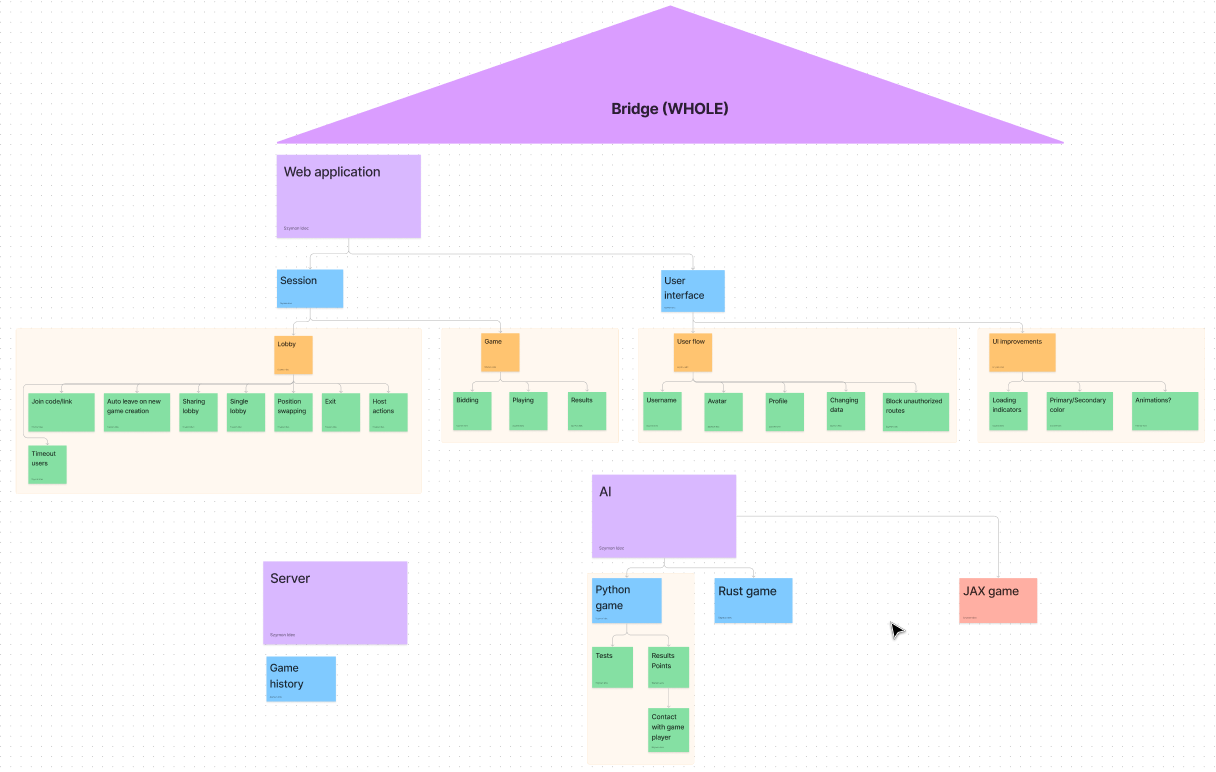
\includegraphics[width=0.9\textwidth]{img/schematy/milestones.png}
  \caption{Szczegółowy podział milestone'ów na zadania}
  \label{fig:figma_strategicplan}
\end{figure}

Opierając się na powyższym planie, można stwierdzić, że udało się
zrealizować wszystkie wymagania sprecyzowane przez klienta.
Jedynym elementem, który został zrealizowany alternatywnie,
zgodnie z~założeniami zagrożeń implementacji
(\nameref{sec:analiza_zagrozen}), był wirtualny asystent. Szczegóły
dotyczące tej części projektu zostały opisane w~sekcji dotyczącej
asystenta \nameref{subsubsec:mocai}.

\section{Przegląd zrealizowanych funkcjonalności}

Poniższa sekcja opisuje wyniki zrealizowanego przez zespół
projektu. Przedstawiona jest aplikacja oraz wyniki, jakie
osiąga wirtualny asystent.

\subsection{Interfejs aplikacji}

Interfejs aplikacji był tworzony z~uwagą na postawione wymagania funkcjonalne.
Zapewnia on użytkownikowi dostęp do wszystkich funkcji niezbędnych do korzystania
z~aplikacji. Widoki aplikacji są w~znacznym stopniu podobne do szkiców wykonanych na etapie
rozpoczęcia prac. Różnią się nieznacznie stylem ze względu na użycie innych narzędzi
do ich utworzenia. Są też bardziej szczegółowe od szkiców, ponieważ nie planowano
rozmieszczenia najdrobniejszych elementów interfejsu, takich jak przyciski akcji hosta
w~lobby czy oznaczenia pozycji graczy na ekranie gry. Przykładowe porównania końcowych
rezultatów ze szkicami są przedstawione na rysunkach \ref{fig:compare_lobby}
i~\ref{fig:compare_game}.

\begin{figure}[h!]
  \centering
  \subfloat[Ekran lobby]{
    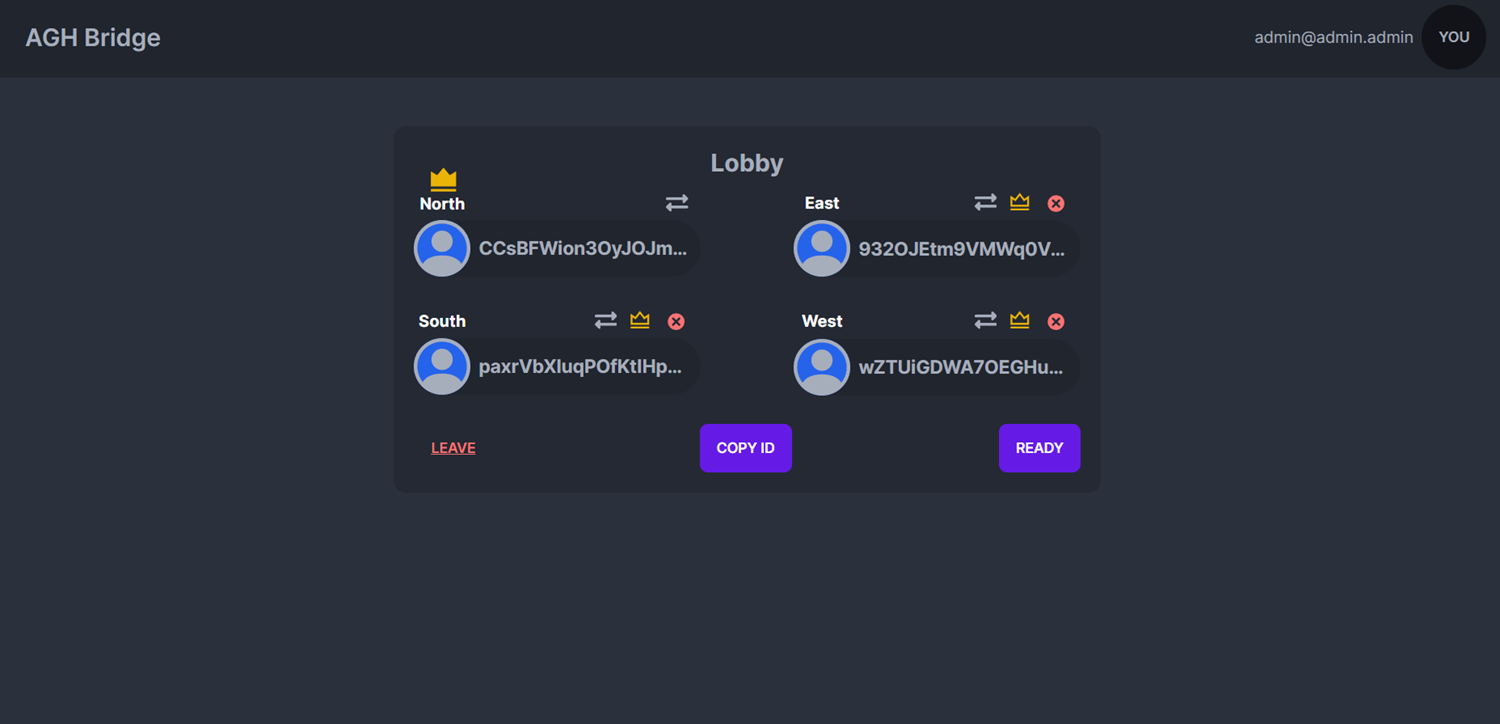
\includegraphics[width=0.45\textwidth]{img/widoki/lobby.png}
  }%
  \hspace*{0.5cm}
  \subfloat[Szkic lobby]{
    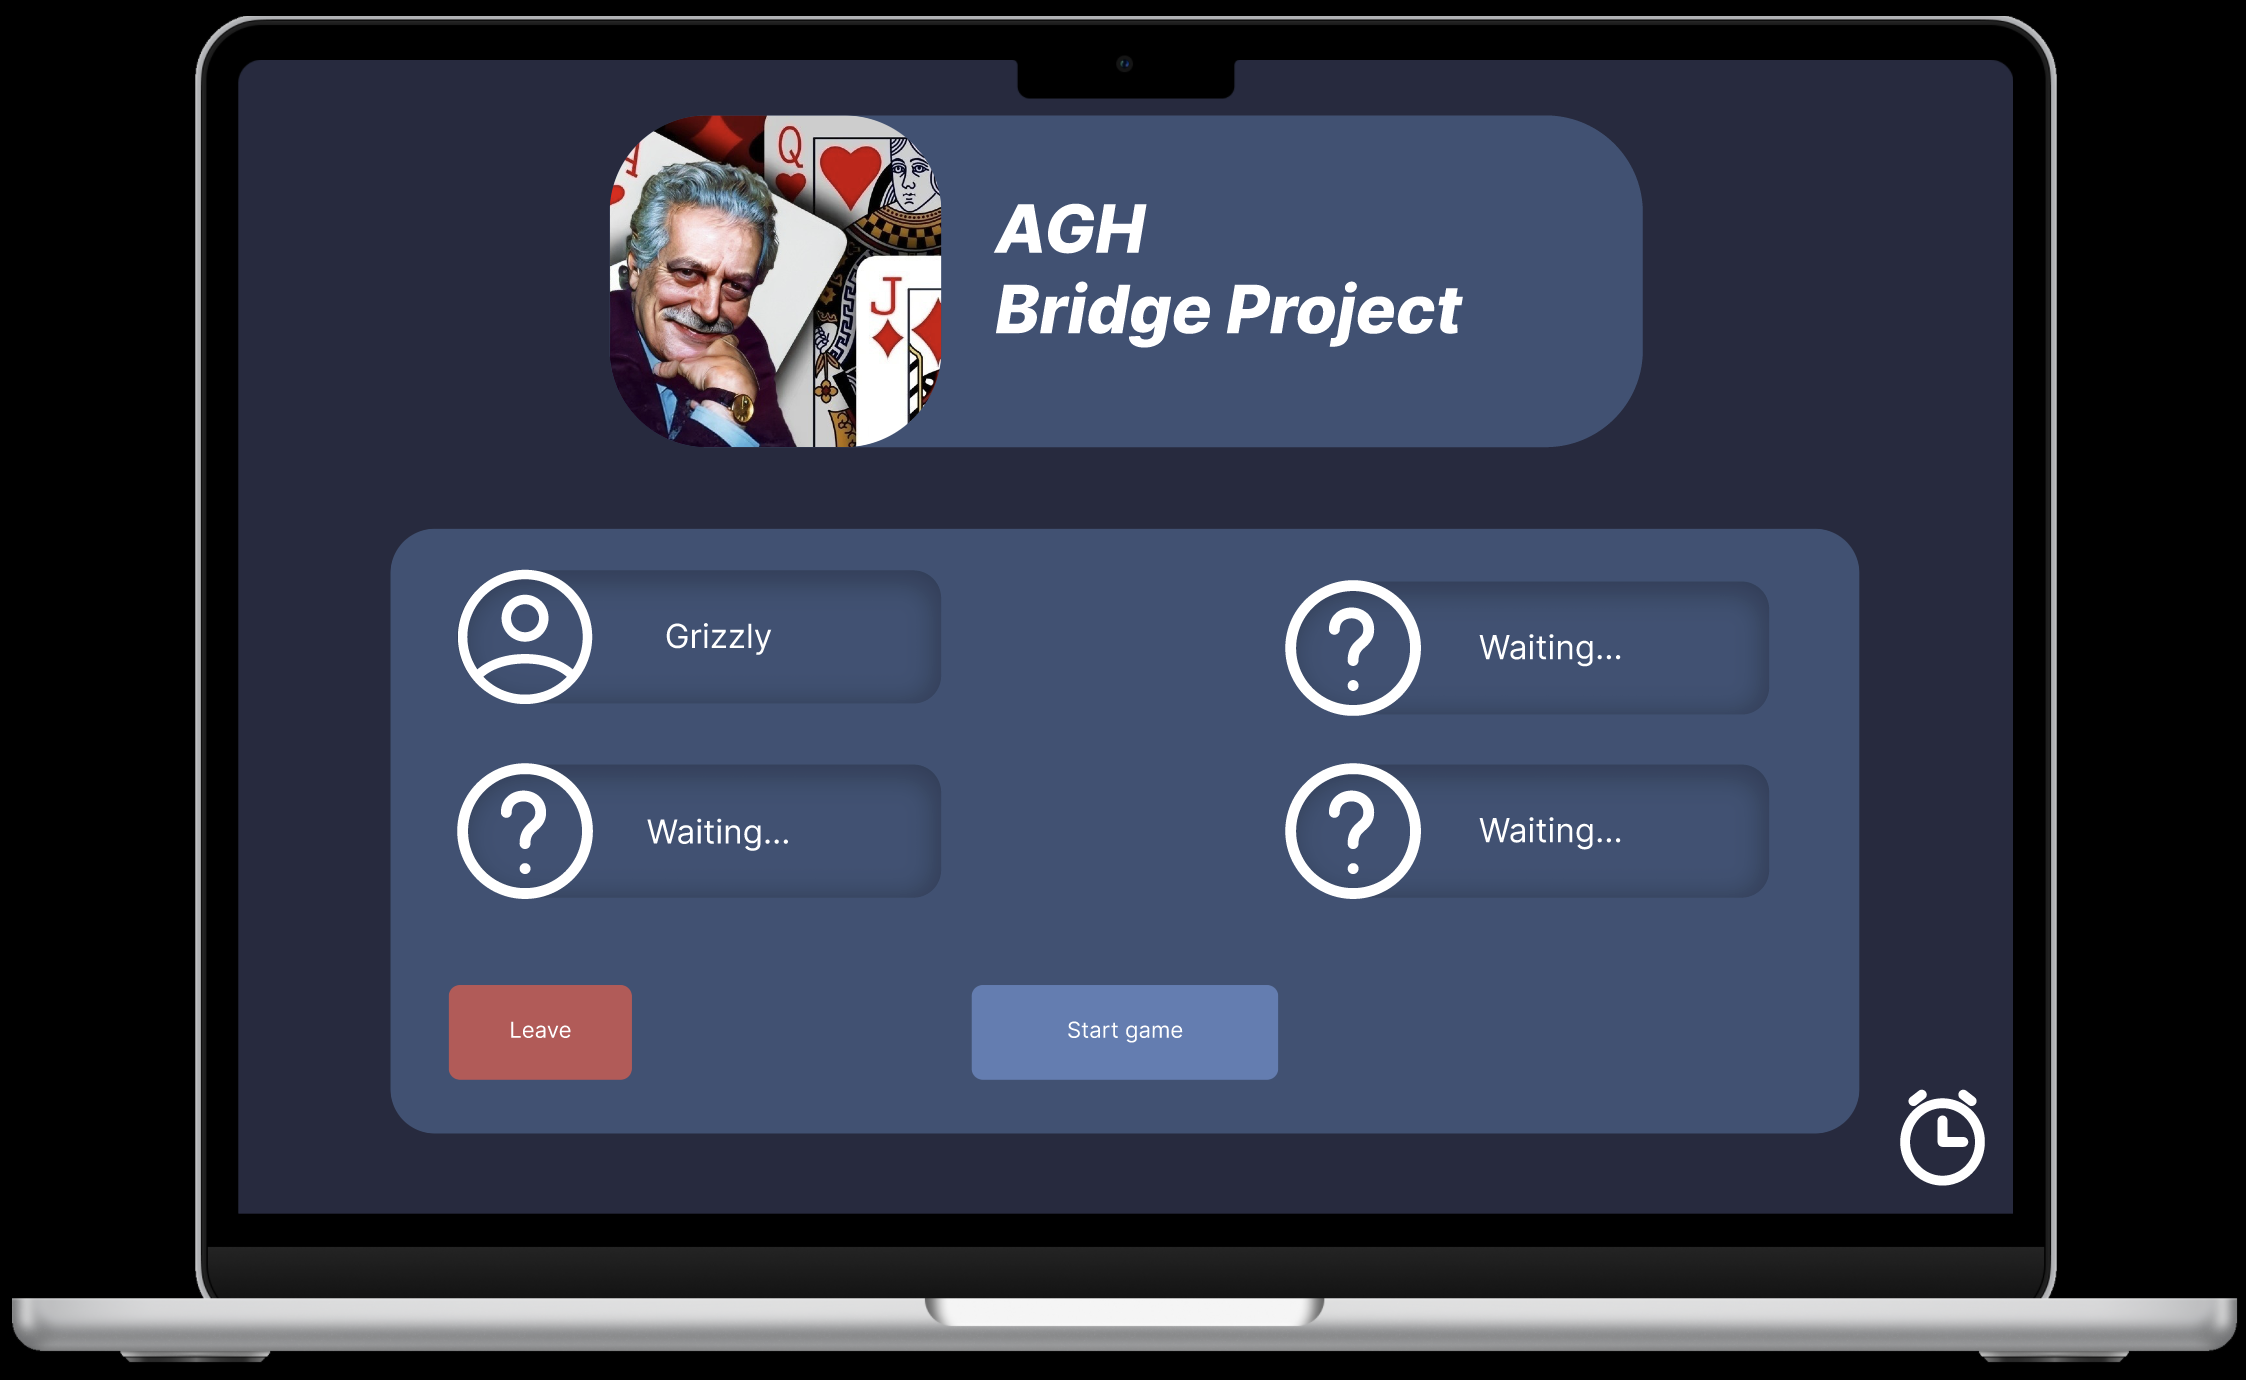
\includegraphics[width=0.45\textwidth]{img/figma-szkic/3.png}
  }%
  \caption{Porównanie ekranu lobby z początkowym szkicem}
  \label{fig:compare_lobby}
\end{figure}

\begin{figure}[h!]
  \centering
  \subfloat[Ekran gry]{
    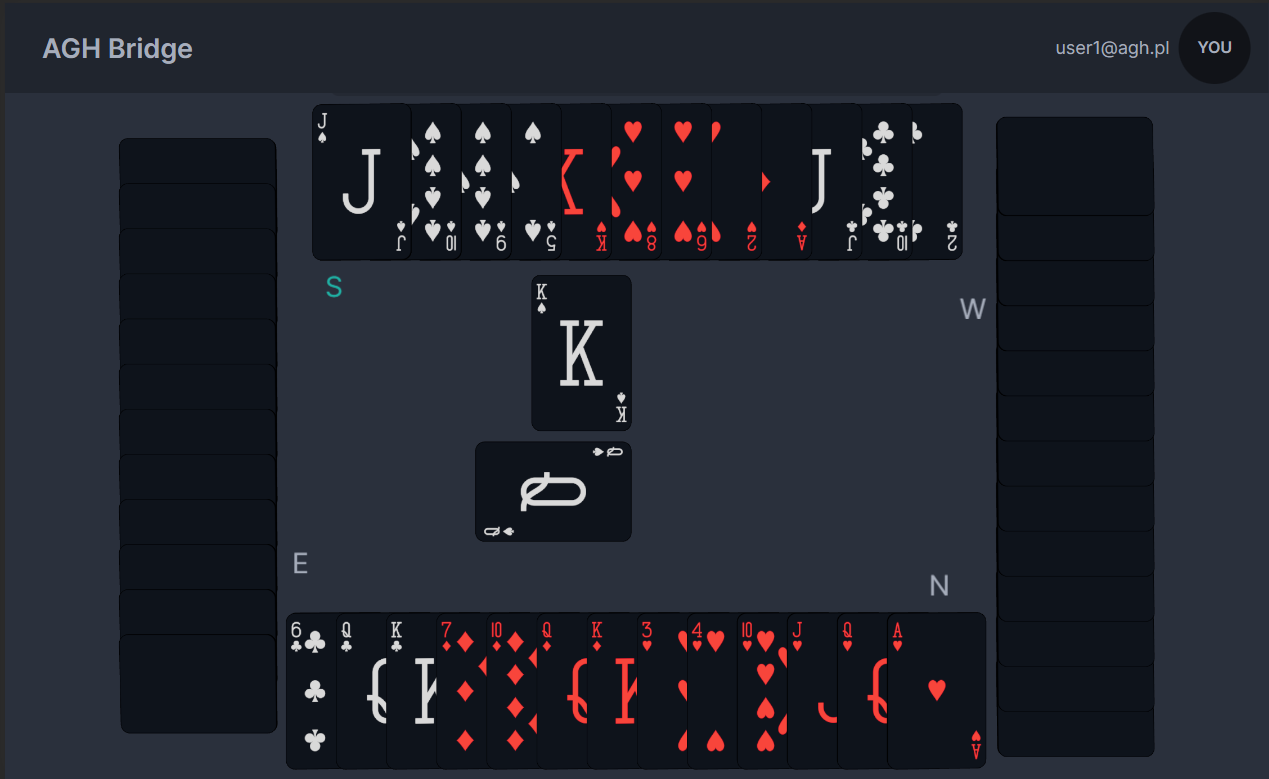
\includegraphics[width=0.45\textwidth]{img/widoki/game.png}
  }%
  \hspace*{0.5cm}
  \subfloat[Szkic gry]{
    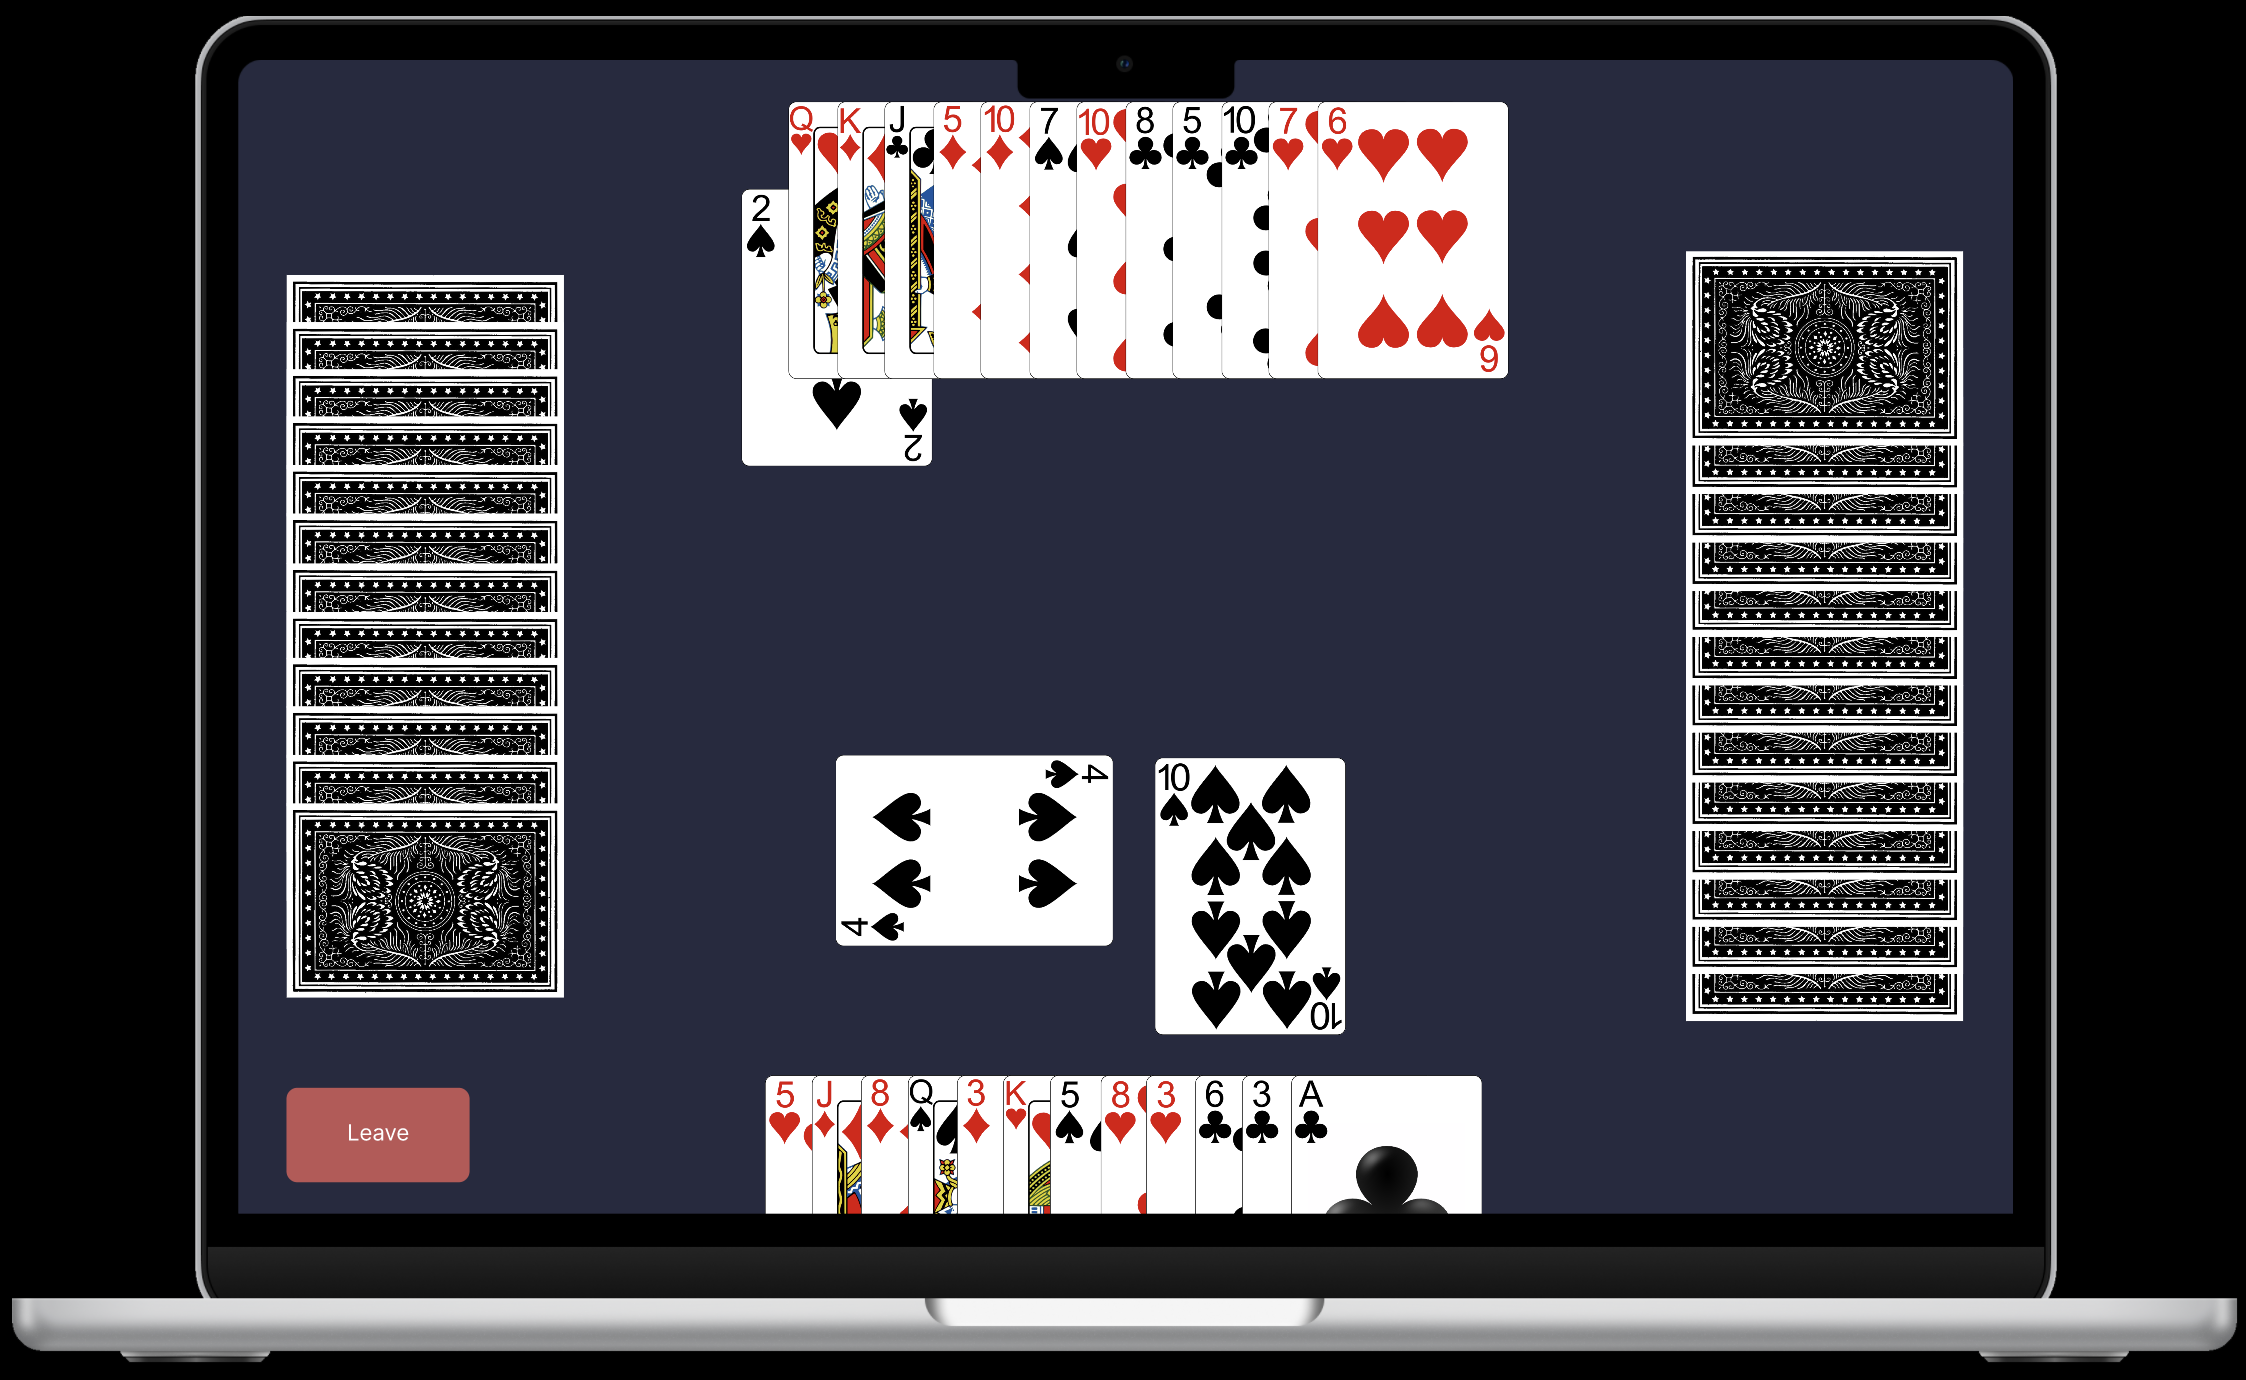
\includegraphics[width=0.45\textwidth]{img/figma-szkic/4.png}
  }%
  \caption{Porównanie ekranu gry z początkowym szkicem}
  \label{fig:compare_game}
\end{figure}

\FloatBarrier

\subsubsection{Tworzenie i dołączenie do gry}

Na stronie głównej aplikacji (Rys. \ref{fig:home}) użytkownik może utworzyć nową
rozgrywkę poprzez naciśnięcie przycisku "Create a game" lub dołączyć do istniejącej
poprzez wpisanie kodu gry otrzymanego od innego użytkownika i~naciśnięcie
przycisku "Join".

\begin{figure}[h!]
  \centering
  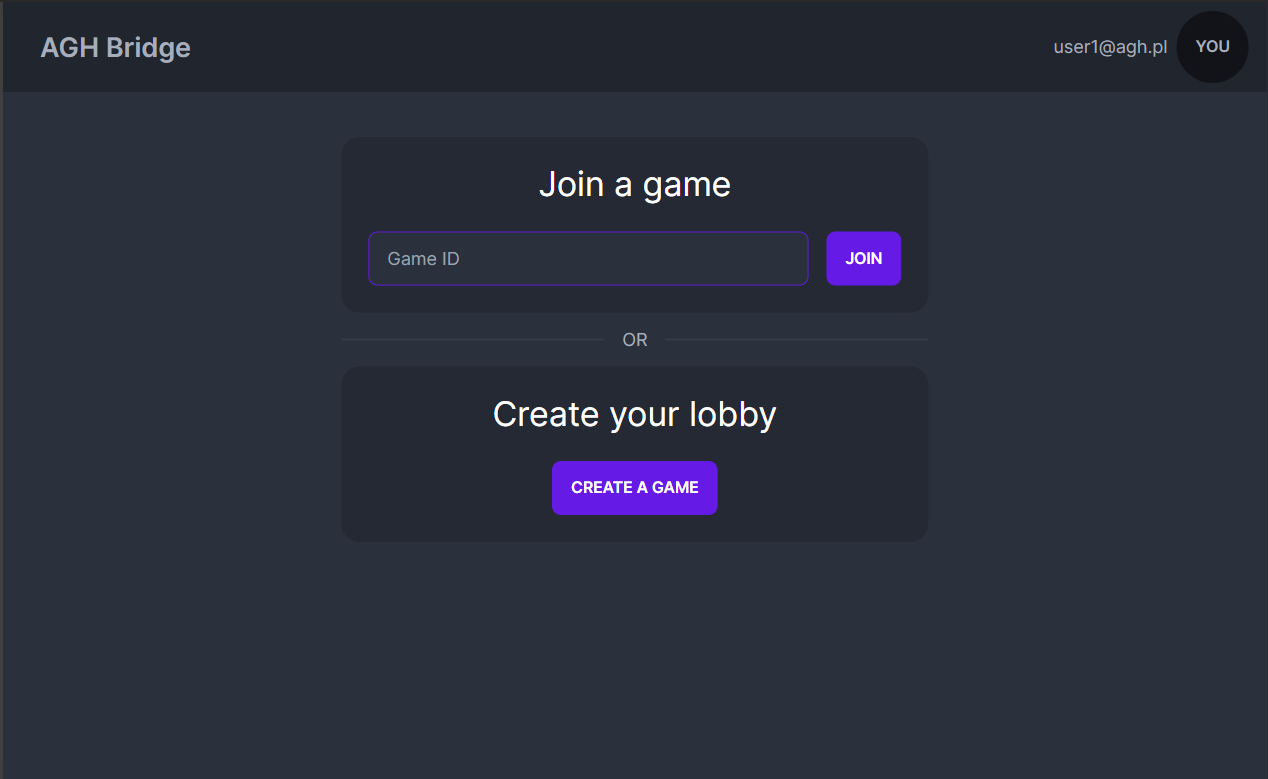
\includegraphics[width=0.9\textwidth]{img/widoki/home.png}
  \caption{Strona główna aplikacji}
  \label{fig:home}
\end{figure}

\FloatBarrier

\subsubsection{Lobby}

Strona lobby (Rys. \ref{fig:lobby}) służy do zebrania
użytkowników przed rozpoczęciem gry i~ustawienia ich
na odpowiednich pozycjach. Widok zawiera cztery pozycje
z~pseudonimami graczy, którzy się na nich znajdują.
Host jest oznaczony ikoną korony, znajdującą się nad nazwą
jego pozycji.

\begin{figure}[h!]
  \centering
  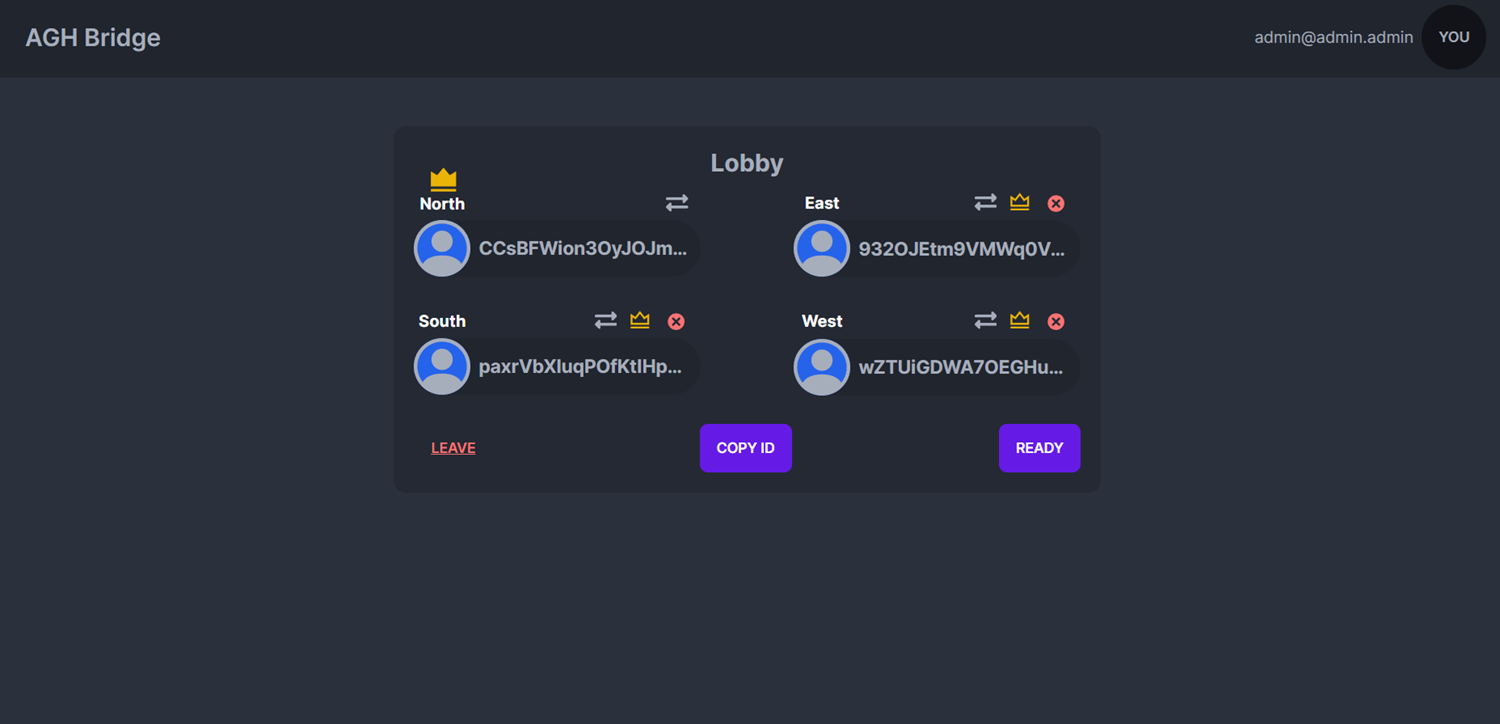
\includegraphics[width=0.9\textwidth]{img/widoki/lobby.png}
  \caption{Strona lobby}
  \label{fig:lobby}
\end{figure}

\FloatBarrier

\subsubsection{Host}

Zgodnie z~założeniami, host ma możliwość wyrzucania graczy
z~lobby, zmieniania ich pozycji oraz obsadzania pustych
miejsc graczami-asystentami. Ponadto, host może oddać swoje
uprawnienia innemu graczowi-użytkownikowi. Te akcje może
wykonywać poprzez użycie odpowiednich przycisków w~postaci
ikon znajdujących się nad pozycjami graczy (Rys. \ref{fig:host_actions_ui}).

\subsubsection{Użytkownik}

Użytkownik ma możliwość w~dowolnym momencie opuścić lobby, naciskając przycisk "Leave",
oraz zgłosić gotowość do rozpoczęcia rozgrywki, poprzez naciśnięcie przycisku "Ready".
Dodatkowo może skopiować kod gry za pomocą przycisku "Copy ID" i~przesłać go innemu
użytkownikowi. Warto zaznaczyć, że kod nie jest widoczny w~żadnym momencie, co może być
przydatne dla graczy udostępniających ekran podczas rozgrywki, aby zabezpieczyć się przed
nieproszonymi uczestnikami.

\subsection{Gra w brydża}

Utworzony został prosty interfejs gry, który zapewnia
wymagane elementy gry jak system licytacji i~widoczne
karty odpowiednich graczy. Ograniczono się głównie do
zaimplementowania tych akcji, jakie mógłby wykonać także
wirtualny asystent.

\subsubsection{Licytacja}

Podczas licytacji użytkownik może na bieżąco obserwować
podejmowane kontrakty przez innych graczy. Niedostępne akcje
są blokowane, co ułatwia wybór odpowiedniego kontraktu.
Wskazywany jest również gracz, który w~danym momencie
mógłby wygrać licytację, gdy trzech kolejnych graczy
pasuje. Przykładowy stan licytacji widoczny jest na rysunku
\ref{fig:bidding}.

\begin{figure}[h!]
  \centering
  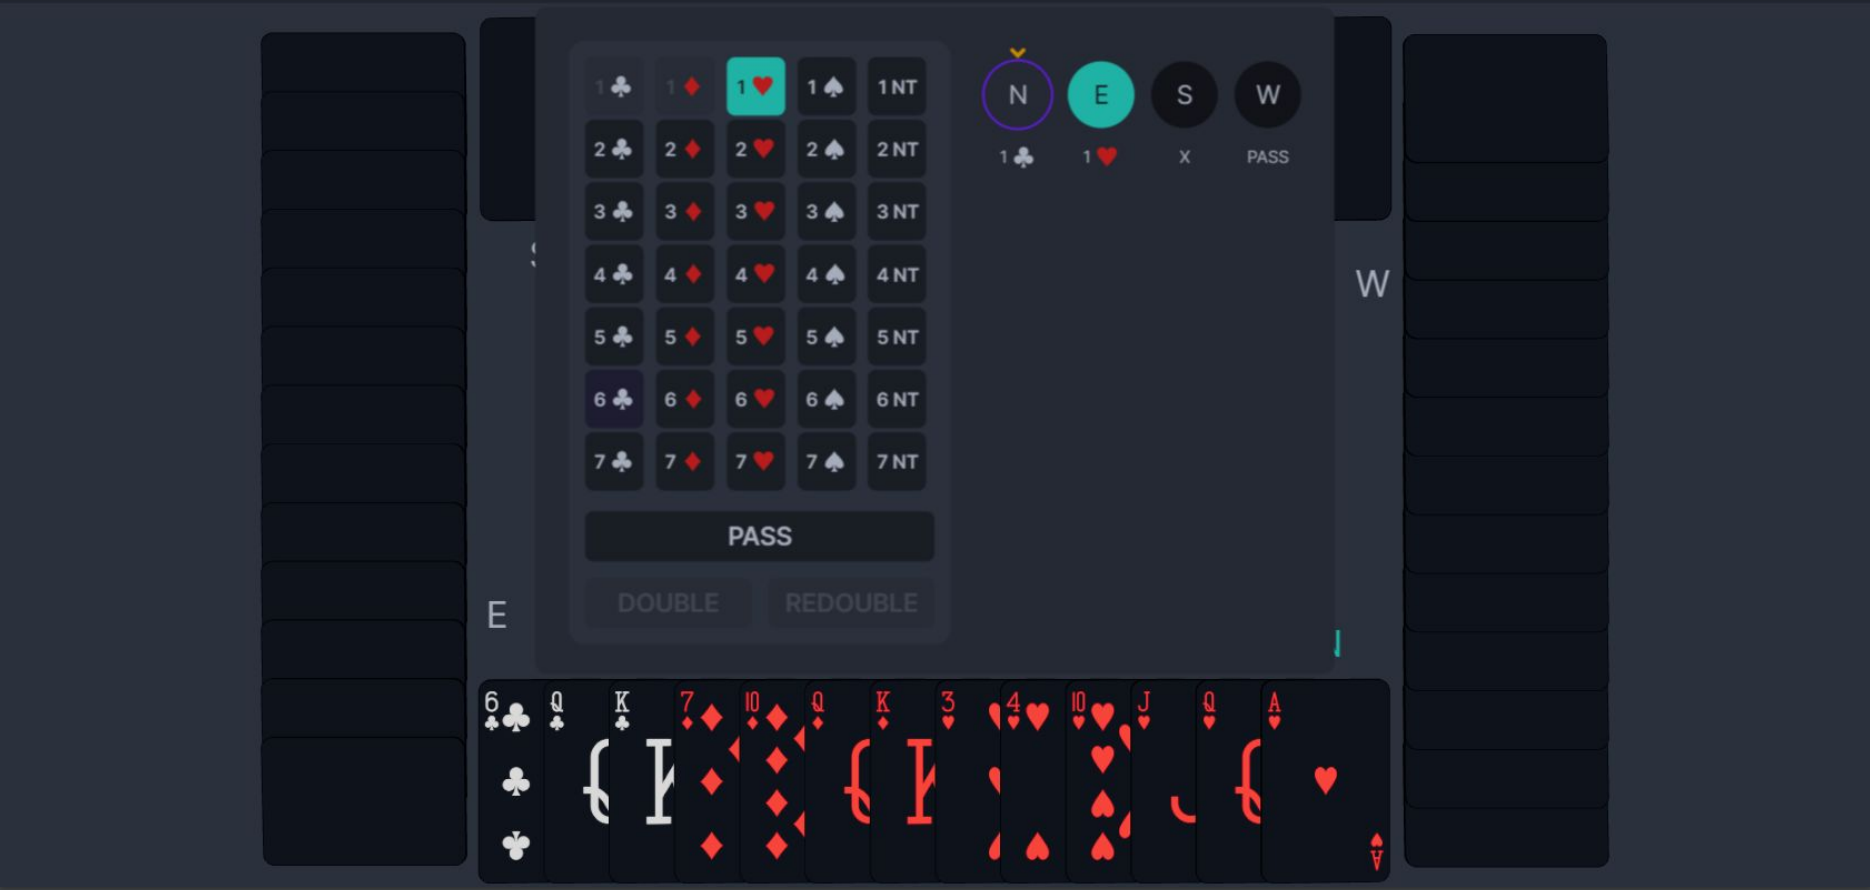
\includegraphics[width=0.9\textwidth]{img/widoki/bidding.png}
  \caption{Interfejs gry podczas licytacji}
  \label{fig:bidding}
\end{figure}

\FloatBarrier

\subsubsection{Rozgrywka}

W~ekranie rozgrywki (Rys. \ref{fig:game}) znalazły się takie
elementy jak widok
kart każdego z~graczy, w~tym widoczne są awersy kart
użytkownika i~dziadka (lub partnera, gdy użytkownik jest
dziadkiem). Litery znajdujące się przy kartach określają
kierunek, na którym się znajdują. Podświetlany jest
kierunek tego gracza, który aktualnie wykonuje ruch.
Na środku ekranu znajdują się zagrane karty tworzące lewę.
Wszystkie karty i~ich zagrania są płynnie animowane,
dzięki czemu użytkownicy mogą doświadczyć gry
w~podobny sposób jak przy prawdziwym stole.

\begin{figure}[h!]
  \centering
  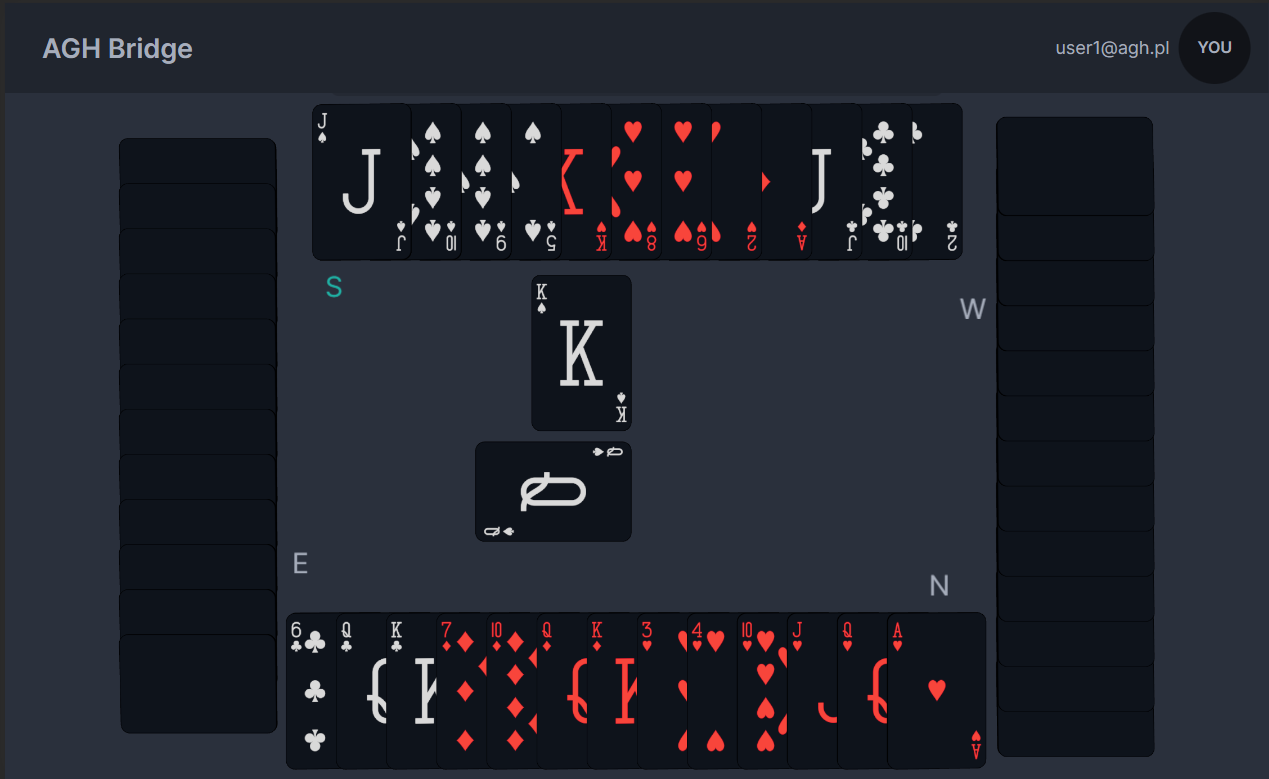
\includegraphics[width=0.9\textwidth]{img/widoki/game.png}
  \caption{Interfejs gry podczas rozgrywki}
  \label{fig:game}
\end{figure}

\FloatBarrier

\subsection{Wirtualny asystent}
%%% przeprowadzone testy aplikacji na wybranej grupie osób (do wywalenia?)

W fazie planowania projektu wskazano 5 różnych algorytmów AI, które mogłyby zostać
wykorzystane.
Nie podjęto próby implementacji pierwszego z nich (Regularized Nash Dynamics),
ze względu na jego złożoność i~brak dostępnych implementacji.
Zdecydowano się na implementację drugiego algorytmu (AlphaZero).
Początkowo planowano wykorzystanie rozszerzenia IS-MCTS.
Odkryto jednak sposób na zaimplementowanie algorytmu bez tego rozszerzenia,
co pozwoliło na uproszczenie implementacji. Nazywamy tę wersję algorytmu
\textit{Depth-Zero AlphaZero}.


\subsubsection{Poziom sztucznej inteligencji}
\label{subsubsec:mocai}

Agent AlphaZero uczony był poprzez granie sam ze sobą.
W~procesie uczenia zaobserwował ponad 110~mln ruchów,
co odpowiada około 10 mln gier, zakładając średnią
długość licytacji 11 ruchów.
W~celach ewaluacji agenta, przeprowadzane
były gry pomiędzy agentem a~graczem wykonującym
losowe ruchy.
Nie jest to najlepszy przeciwnik, ale pozwala
ocenić, czy agent polepsza swoje umiejętności.
Ewaluacja wykorzystywała samą sieć $\mathbf{p}$,
agent nie widział kart innych graczy.
Wyniki przedstawia Rys. \ref{fig:bzero-eval}.
Agent szybko osiąga 95\% wygranych.
Brak 100\% wygranych wynika z~faktu, że
podczas ewaluacji agent nie wybiera zawsze optymalnego ruchu,
tylko losuje ruch z~rozkładu prawdopodobieństwa
wygenerowanego przez $\mathbf{p}$.
Służy to zróżnicowaniu gier i~umożliwia
dokładniejszą ocenę umiejętności agenta.


\begin{figure}[!]
  \centering
  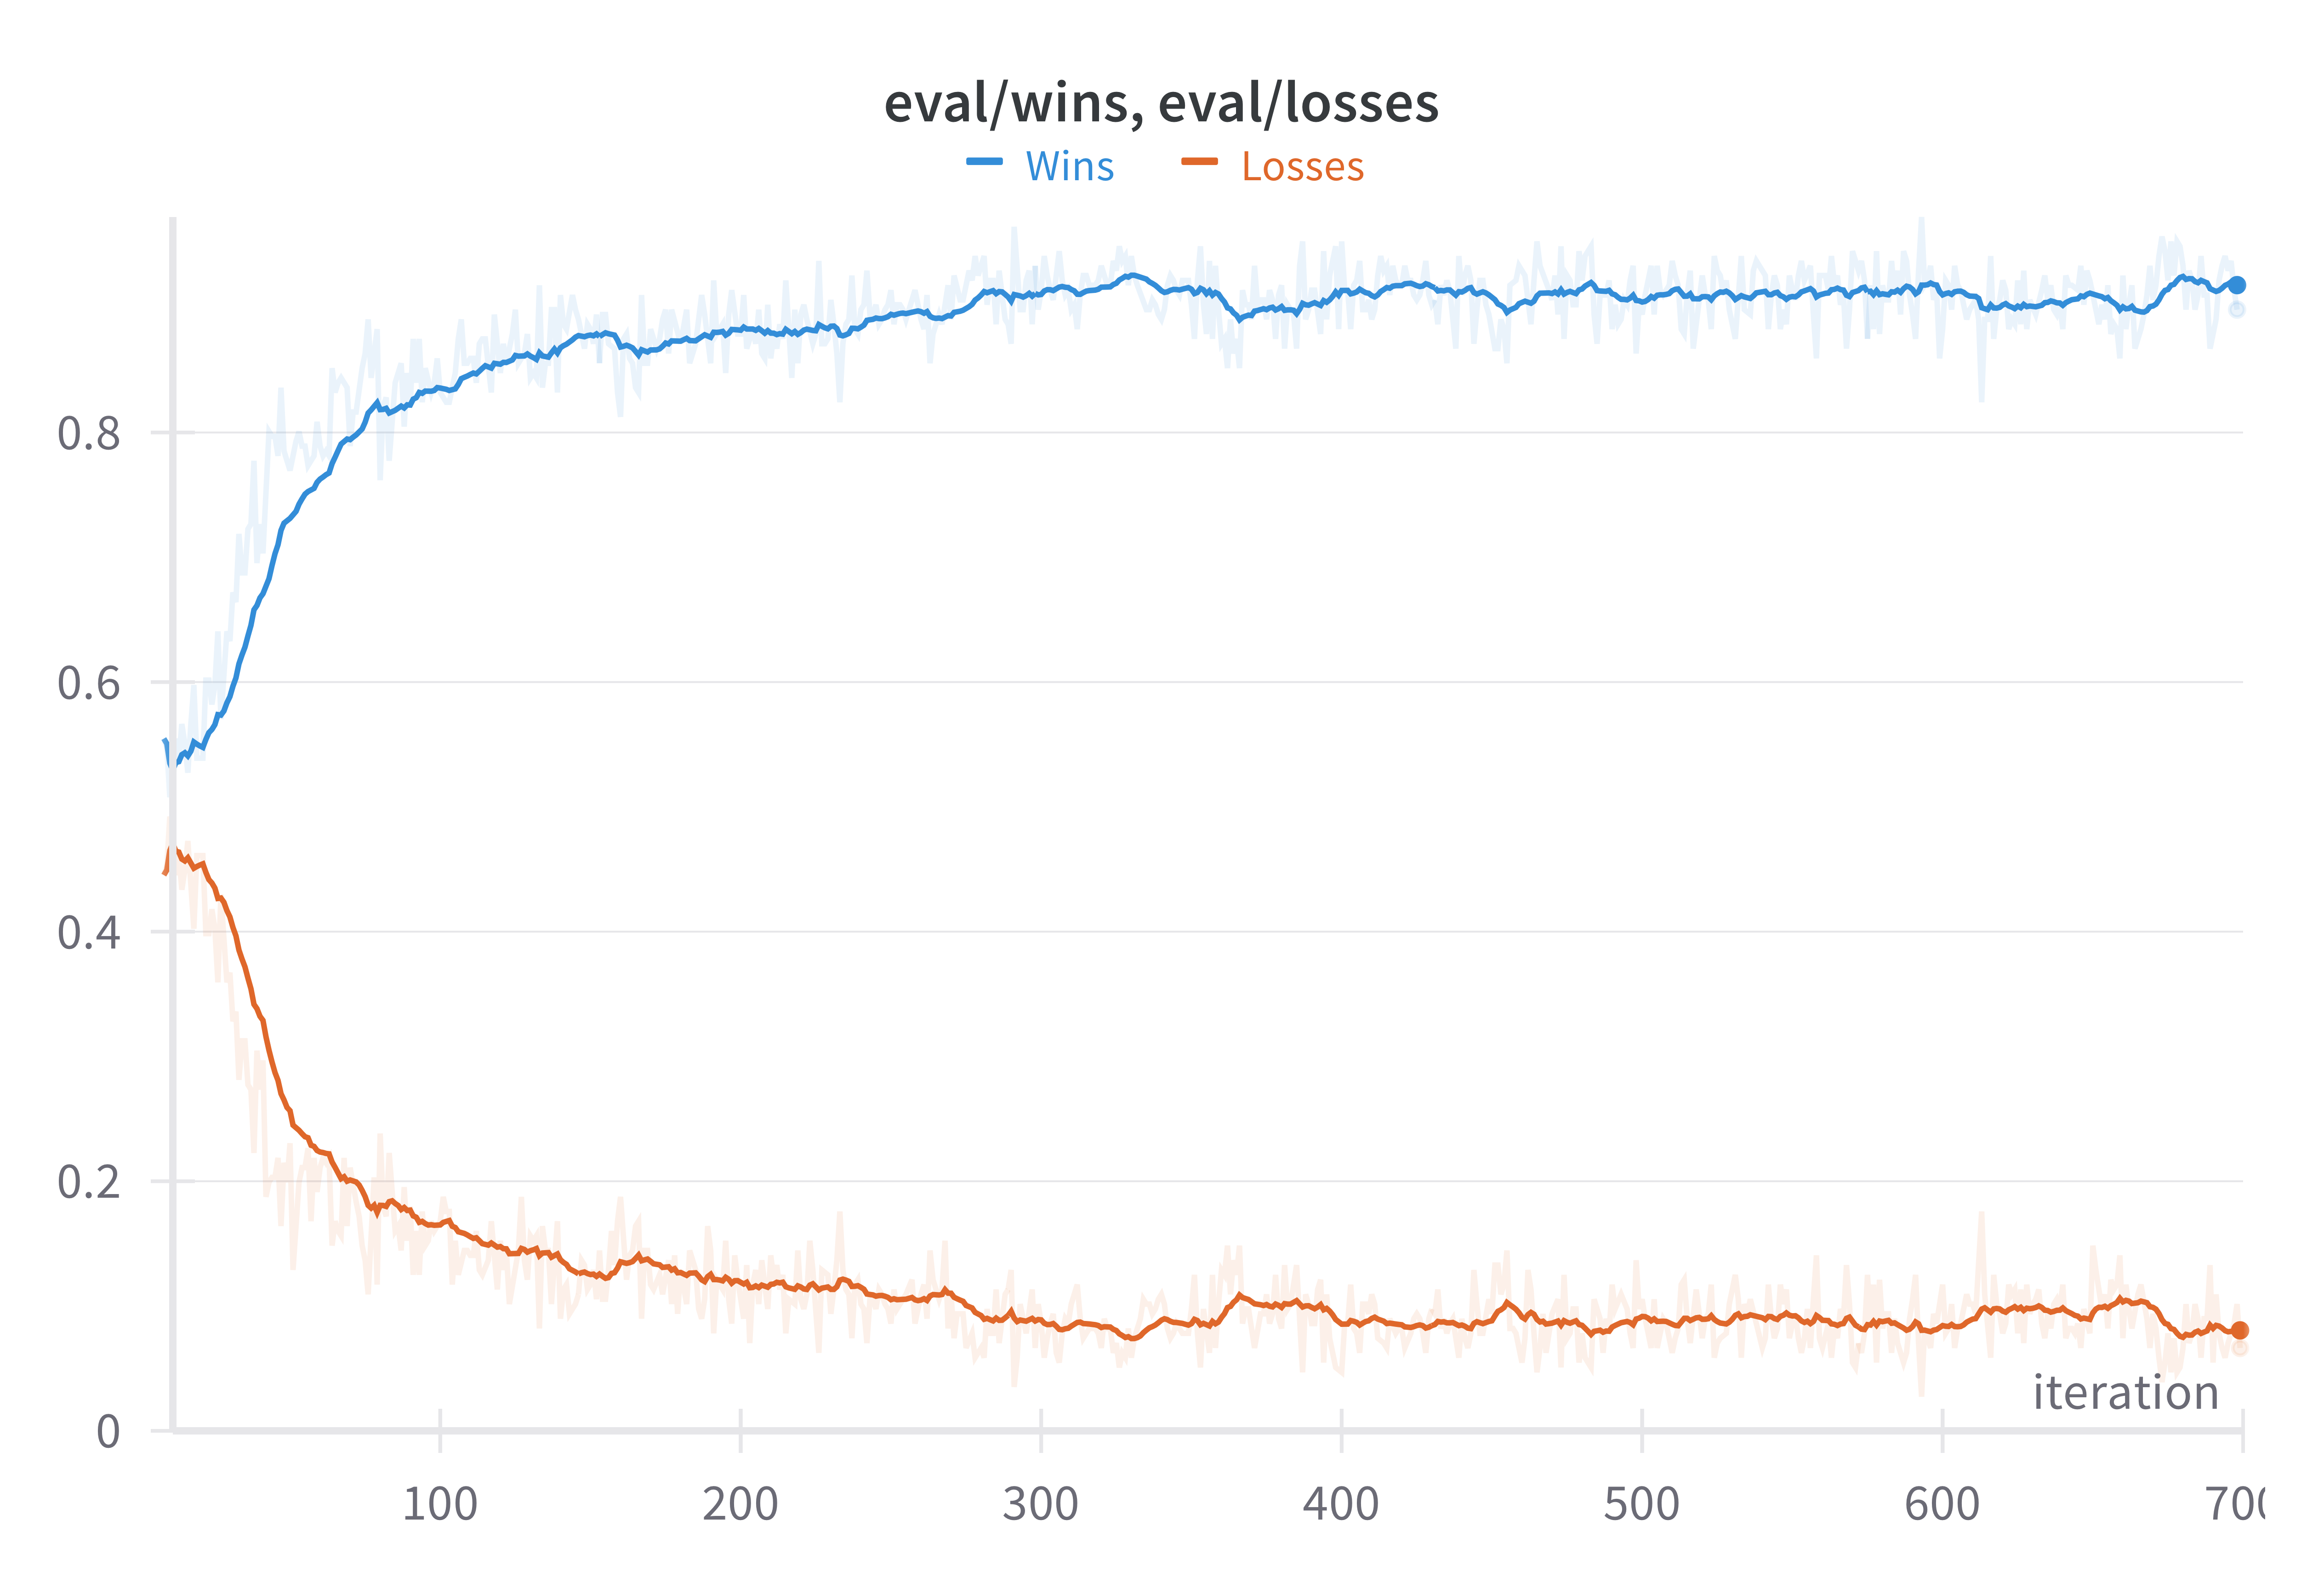
\includegraphics[width=\textwidth]{img/wykresy/bzero-eval.png}
  \caption{Proces uczenia AlphaZero vs. losowy gracz -- Licytacja}
  \label{fig:bzero-eval}
\end{figure}

\begin{figure}[!]
  \centering
  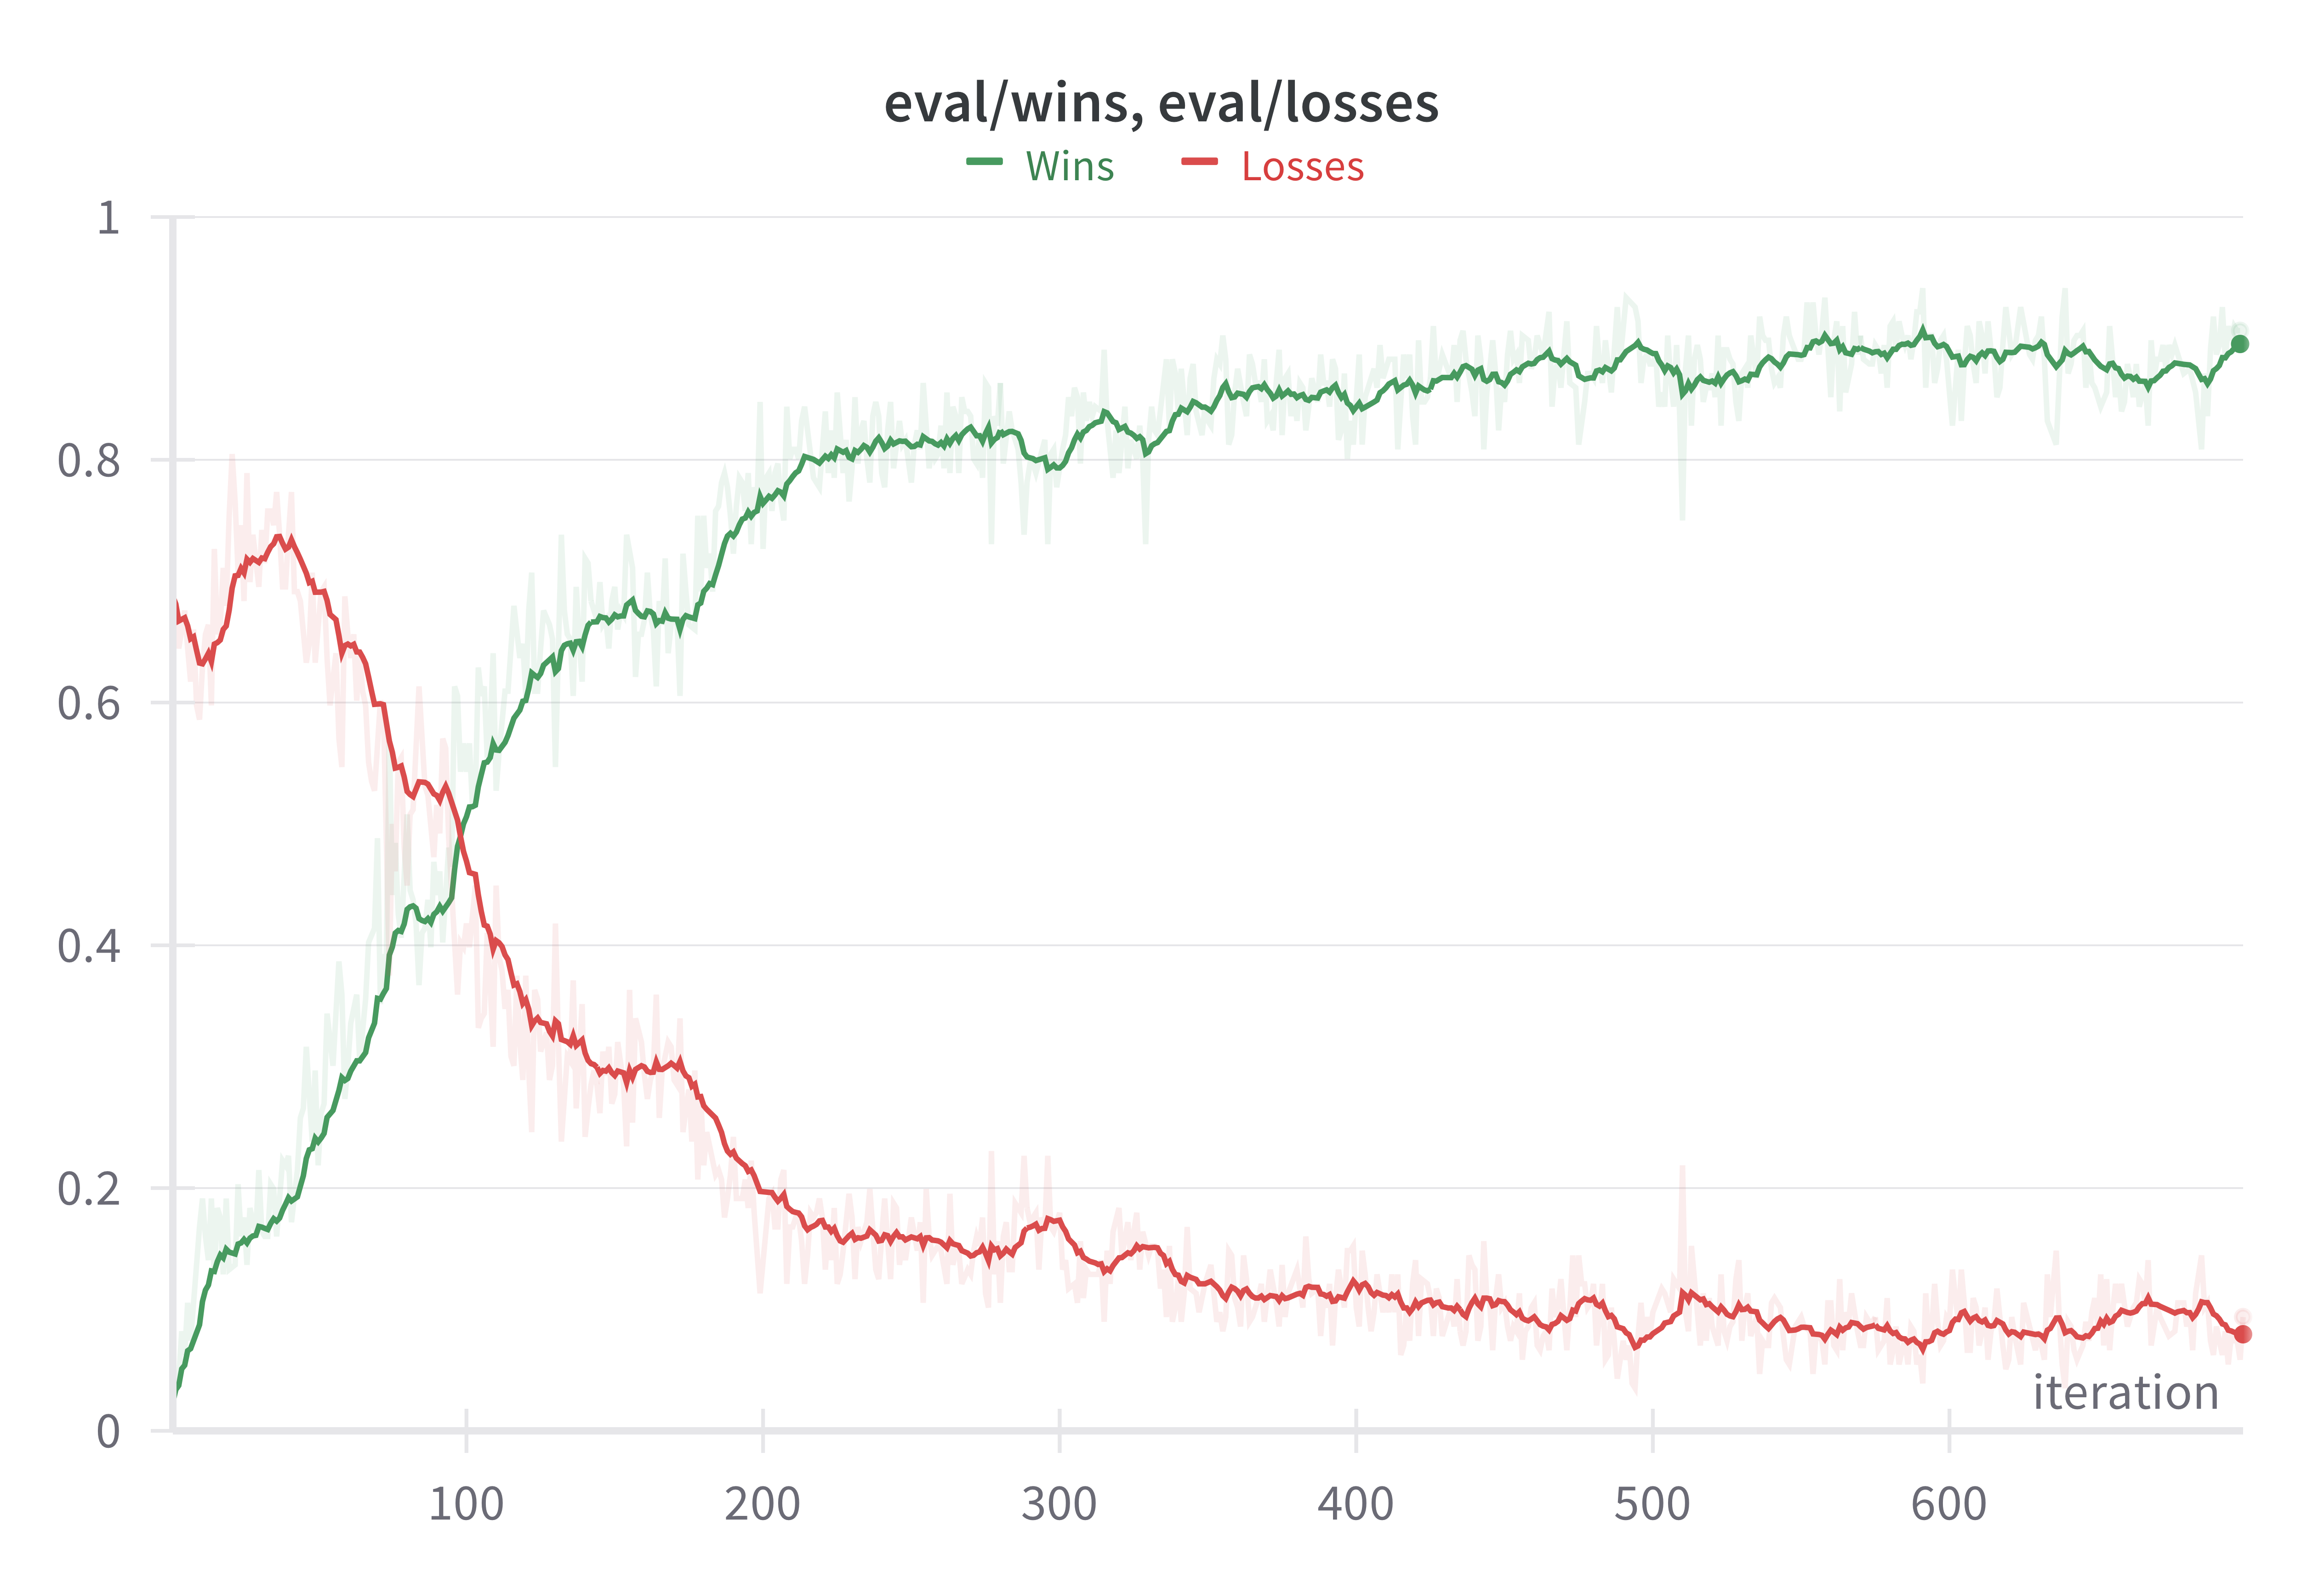
\includegraphics[width=\textwidth]{img/wykresy/othello-eval.png}
  \caption{Proces uczenia AlphaZero vs. PGX Baseline -- Othello}
  \label{fig:othello-eval}
\end{figure}

Ze względu na brak odpowiedniego modelu
bazowego (baseline) przeciwnika,
przeprowadzono test zaimplementowanego algorytmu
na grze Othello \cite{Othello}.
Uruchomiono identyczny proces uczenia,
wykorzystując implementację Othello oraz
model AI baseline z~\cite{PGX}.
Wyniki uczenia przedstawia Rys.~\ref{fig:othello-eval}.
Nasze AI uzyskuje stosunek wygranych do przegranych
kontra model AI baseline na poziomie 9:1.
Można zatem wnioskować, że nasza implementacja
AlphaZero jest poprawna.

AI do fazy rozgrywki wykorzystuje algorytm DDS,
zatem jest matematycznie doskonałe i~nie ma potrzeby
oceny jego umiejętności.

\FloatBarrier

\subsubsection{Możliwości rozwoju modelu}
%%% czy da sie rozszerzac o kolejne elementy gry brydza
%%% mozna sie odwolac do dalszych perspektyw (na ten moment w PR)

Efektem implementacji AlphaZero było stworzenie
rozbudowanego środowiska do uczenia.
W~przyszłości można wykorzystać to środowisko
do uczenia innych algorytmów AI, między innymi
Regularized Nash Dynamics.
Znaczna część kodu jest wspólna dla obu algorytmów.
W~przyszłości można również rozszerzyć
model o~dodatkowe elementy gry w~brydża,
na przykład o~systemy licytacyjne.



\subsection{Ułatwienia dostępności}

Oprócz omówionych kluczowych funkcjonalności, w~ramach rozwoju
aplikacji wprowadzono także dodatkowe elementy, których
potrzebę przedstawiono w~podrozdziale dotyczącym wymagań
niefunkcjonalnych. Głównych ich celem było zapewnienie
wygody i~prostego korzystania z~aplikacji, nawet podczas
pierwszego użytkowania. Poniżej przedstawione rozwiązania powstały
z~inicjatywy zespołu. Zostały one zaakceptowane przez klienta,
realizując wymagania dostępności i~użyteczności.

\subsubsection{Intuicyjność interfejsu}

Aby aplikacja była intuicyjna dla każdego użytkownika,
zastosowano ikony wprost kojarzące się z~wykonywaną
przez nie akcją. Zastosowano wyróżniające się kolory wśród palety
aplikacji w~celu podkreślenia danych czynności wykonywanych
przez użytkownika (Rys. \ref{fig:host_actions_ui}). Kontrastowe barwy mają zwrócić uwagę na
skutki danej akcji. Przykładowo jaskrawy czerwony kolor
kojarzący się przemocą lub impulsywnością wraz z~ikoną
przedstawiającą "$\times$"\xspace odpowiada za wyrzucenie gracza
z~sesji. Zastosowanie wspomnianych technik przestrzega
użytkownika przed przedwczesnym kliknięciem, ale także kojarzą
się one z~negatywną czynnością.

\begin{figure}[h!]
  \centering
  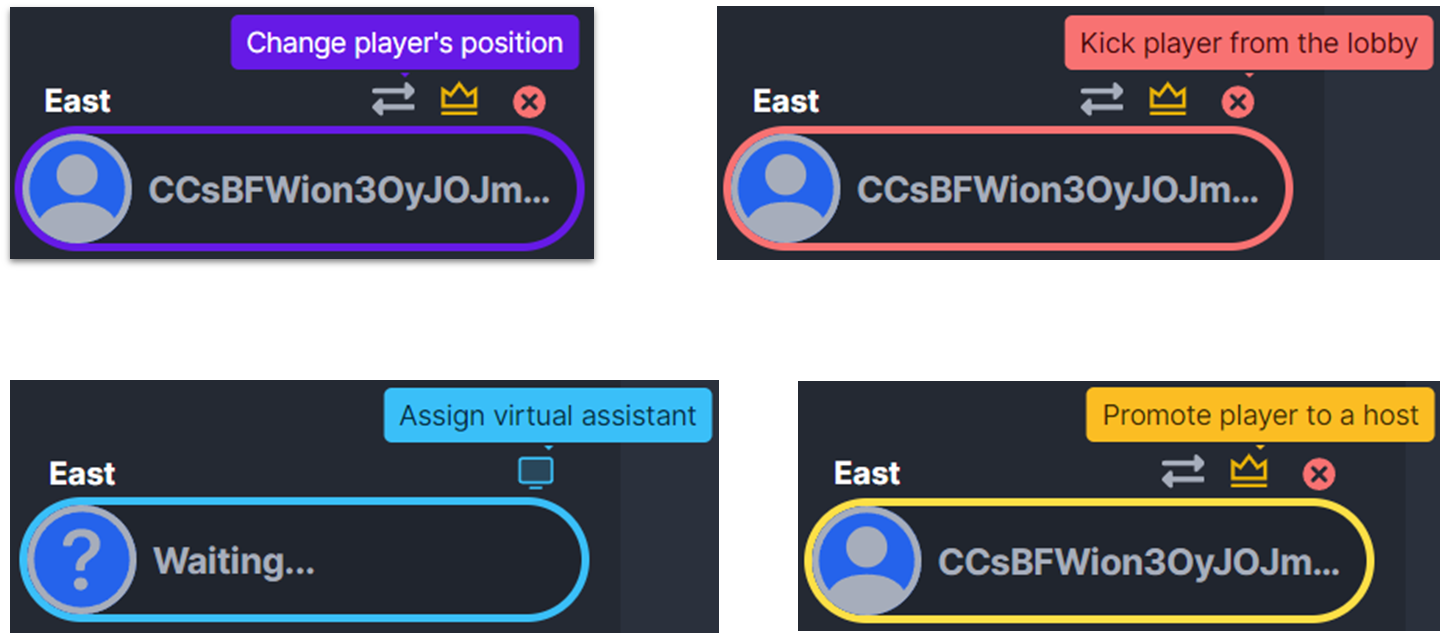
\includegraphics[width=0.9\textwidth]{img/widoki/host_actions.png}
  \caption{Akcje hosta lobby}
  \label{fig:host_actions_ui}
\end{figure}

\FloatBarrier

\subsubsection{Responsywny układ aplikacji}

Zgodnie z~wymogiem dostępności interfejsy aplikacji powinny
być funkcjonalne również na urządzeniach o~niewielkich
rozmiarach ekranu. Wszystkie strony zostały zaprojektowane
tak, aby umożliwić wygodne korzystanie zarówno na urządzeniach
stacjonarnych, jak i~mobilnych (Rys. \ref{fig:responsive_ui}). Aplikacja dynamicznie
dostosowuje się w~zależności od aktualnego rozmiaru okna
przeglądarki.

Minimalna przewidziana
szerokość ekranu wynosi 280 pikseli, dzięki czemu wspierane
są także starsze urządzenia o~niewielkiej rozdzielczości
ekranu.

\begin{figure}[h!]
  \centering
  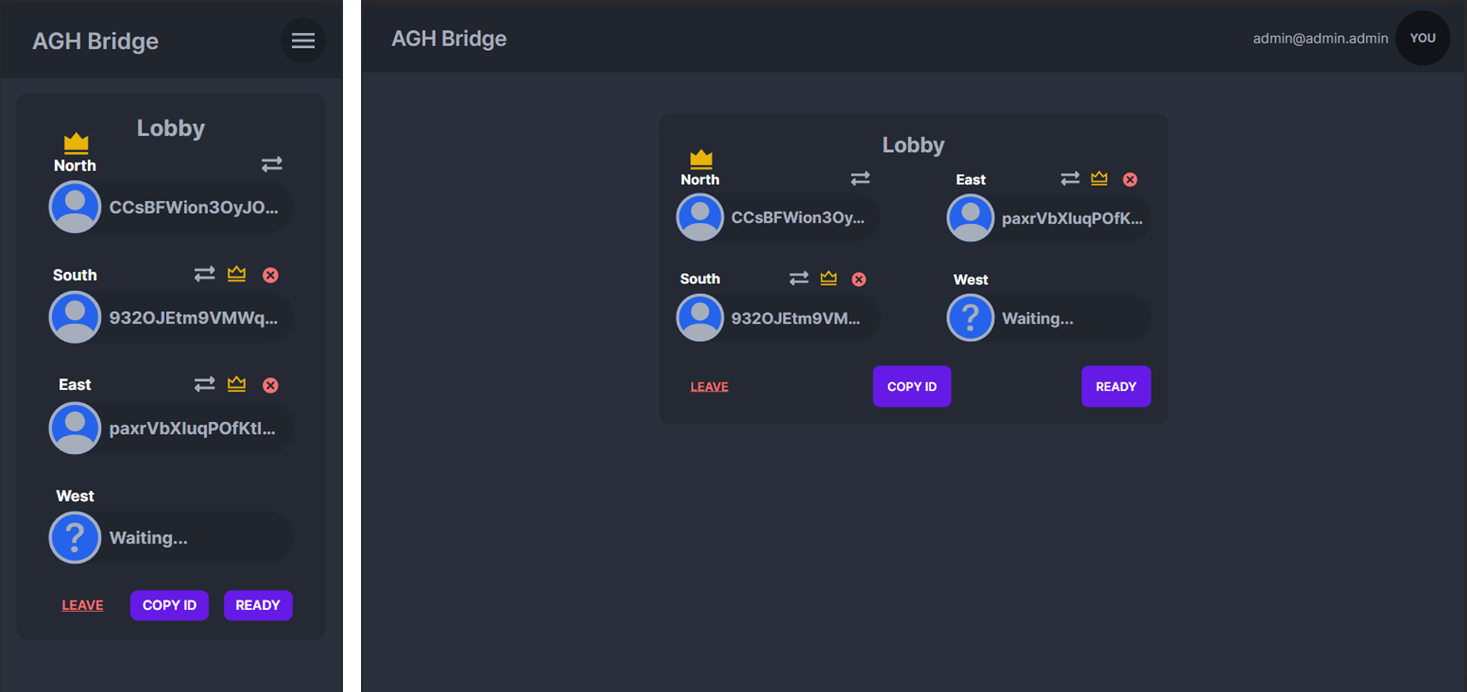
\includegraphics[width=0.9\textwidth]{img/widoki/desktop_mobile.png}
  \caption{Tryb mobilny i desktopowy aplikacji}
  \label{fig:responsive_ui}
\end{figure}

\FloatBarrier

\subsubsection{Motywy jasny i ciemny}

Wygląd aplikacji został zrealizowany w~dwóch trybach --
jasnym i~ciemnym (Rys. \ref{fig:themes_ui}). Użyto w~tym celu dostępnych w~bibliotece
palet kolorów, ale także zdefiniowano własne, aby zachować
motyw kolorystyczny aplikacji. W~zależności od aktualnie
wybranego motywu kolory zmieniały swój odcień.

% \begin{figure}[h!]
%   \centering
%   \includegraphics[width=\textwidth, draft=true]{example-image}
%   \caption{Motywy jasny i ciemny aplikacji}
%   \label{fig:themes_ui}
% \end{figure}

% \FloatBarrier

\begin{figure}[h!]
  \centering
  \begin{minipage}[b]{0.45\textwidth}
    \centering
    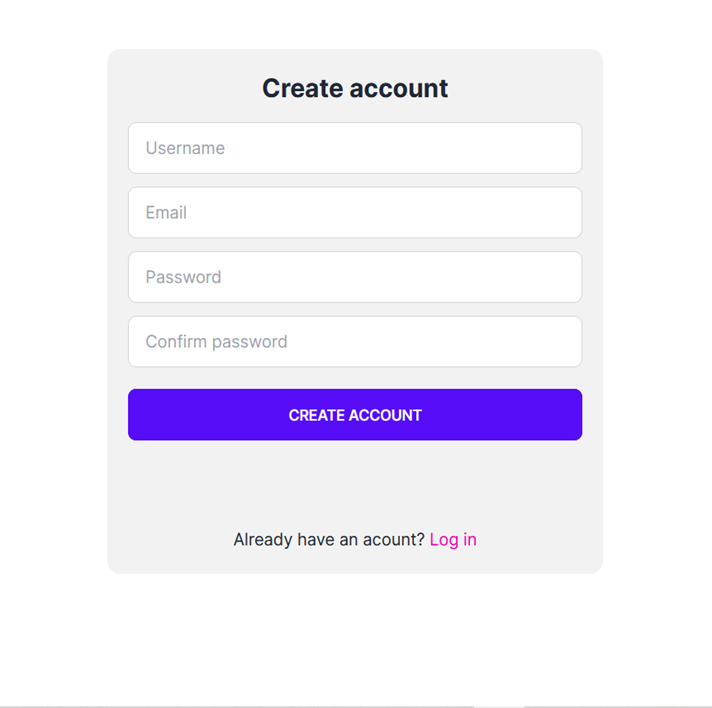
\includegraphics[width=\textwidth]{img/widoki/light.png}
  \end{minipage}%
  \hspace*{0.5cm}
  \begin{minipage}[b]{0.45\textwidth}
    \centering
    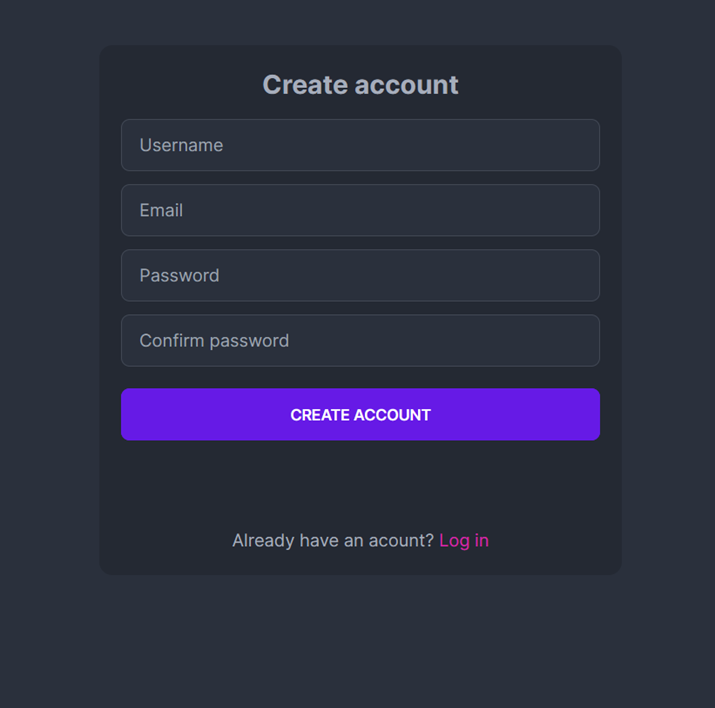
\includegraphics[width=\textwidth]{img/widoki/dark.png}
  \end{minipage}
  \caption{Motywy jasny i ciemny aplikacji}
  \label{fig:themes_ui}
\end{figure}

\FloatBarrier

\section{Dalsze perspektywy rozwoju projektu}

Aplikacja do gry w~brydża została stworzona głównie
na potrzeby asystenta, aby można było go wykorzystać w~grze
poprzez sieć Internet. Tworzona była w~technologiach, które
w~naszej opinii są popularne, a~ich rozwój jest stale wspierany.
Dzięki temu możliwy jest przyszły rozwój lub przebudowa aktualnej
wersji aplikacji.
W~związku z~tym zaproponowano potencjalne funkcjonalności rozszerzające
możliwości asystenta i~aplikacji, które
mogłyby być rozwinięte w~przyszłości. \\

Jedną z~ważniejszych funkcji jest wprowadzenie wsparcia do
przeprowadzenia pełnej rozgrywki gry. Na ten moment możliwe jest
rozegranie jednego rozdania. Przy wprowadzeniu pełnej gry należałoby
utworzyć zapisy wyników z~każdej partii, w~których skład wchodzą rozdania,
a~także dostosować asystenta
do uwzględniania wyników gry\footnote{Uwzględnienie wyników gry jest
  rozumiane jako dodanie wyników gry do obserwacji modelu asystenta.}
podczas podejmowania decyzji. Istotne w~tym przypadku
byłoby również rozszerzenie interfejsu gry, aby mógł zawierać
dodatkowe informacje, jak na przykład aktualny wynik gry lub
historię licytacji.

Również istotną propozycją, która z~pewnością podniesie poziom
współpracy asystenta z~graczem, jest wsparcie języków licytacji\footnote{
  język licytacji -- odzywki licytacyjne mające przekazać informacje
  partnerowi, którym przypisane
  są ustalone informacje o~posiadanych kartach.
} (systemów licytacji).
Aktualnie asystent podejmuje decyzje podczas licytacji bez znajomości
języków. Oznacza to, że nie rozumie odzywek gracza w~stosowanym przez
niego systemie licytacyjnym.

Dodatkową funkcjonalnością, która rozszerza zastosowanie asystenta, jest
wykorzystanie go do analizy rozgrywek w~czasie rzeczywistym lub
ich historycznych zapisów. Dzięki temu gracz mógłby uzyskać podpowiedzi
o~możliwie najlepszych ruchach na podstawie aktualnego stanu gry.
W~przypadku gier już odbytych mógłby także sprawdzić, w~jakich etapach
zostały popełnione błędy lub wykonano najlepsze z~możliwych ruchów.

Również można rozwinąć analizę przeprowadzoną przez asystenta, aby
podpowiedzi do gry były zintegrowane z~modelem językowym. Dzięki
takiemu rozwiązaniu gracz mógłby korzystać z~chatu dostępnego
z~poziomu aplikacji, aby zadać pytanie o~aktualnie przeprowadzanej
rozgrywce lub na temat zasad gry w~brydża. Model językowy zapewniłby
zrozumiałe dla gracza odpowiedzi i~w~razie potrzeby mógłby bardziej
szczegółowo sprecyzować odpowiedź na prośbę gracza.

\section{Podsumowanie}

Uczestnictwo przez zespół w~tworzeniu projektu
było wielkim wyzwaniem dla każdego z~jego członków.
Doświadczyliśmy wielu problemów, z~którymi nie
zmierzyliśmy się wcześniej. Podczas tworzenia
produktu wykorzystaliśmy własne umiejętności nabyte podczas
toku studiów, jak i~sami poznaliśmy wiele nowych technologii.
Odkryliśmy wiele rozwiązań i~sposobów na realizacje
platformy webowej i~udało nam się wdrożyć je do naszej aplikacji.
Rozszerzyliśmy wiedzę z~zakresu połączeń sieciowych, znajdując
rozwiązanie oferujące niskie opóźnienie pomiędzy serwerem gry
a~klientem. Po raz pierwszy zetknęliśmy się z~tworzeniem
środowiska z~zastosowaniem trójwymiarowej grafiki komputerowej
oraz przebadaliśmy wiele informacji dotyczących sztucznej
inteligencji i~możliwości zastosowania jej do tak złożonej gry
jak brydż.

Poprzez analizę
wymagań, planowanie, analizę zagrożeń, implementację
i~testowanie utworzono pełny system spełniający wymagania
klienta.
Stworzona aplikacja jest w~pełni użyteczna i~może być
wykorzystywana w~sposób darmowy do grania w~brydża przez Internet.

Jesteśmy usatysfakcjonowani z~finalnego rozwiązania produktu,
które dostarczyliśmy i~zadowoleni, że udało nam się pokonać
większość trudności podczas jego realizacji.



